\appendix

\chapter{Observations} \label{Sub-Sec: Observations}
\begin{table}[h]
    \centering
    \caption{Observations}
    \resizebox{\textwidth}{!}{
    \begin{tabular}{ccccccccc}
        %\tablenum{1}
        \hline
        \multirow{2}{*}{Target} & \thead{RA (J2000)}& \thead{Decl (J2000)} & \thead{Stellar mass} & \thead{Systemic velocity} & \thead{Disk inclination} & \thead{Disk position angle} & \thead{$T_{bol}^{(6)}$} & \thead{Reference}\\
        \thead{} & \thead{(h m s)} & \thead{($^\circ$ ' ")}& \thead{($\rm M_{\odot}$)} & 
        \thead{(km/s)} & \thead{}& \thead{} & \thead{(K)} & \thead{}\\
        \hline
        Per-emb-2 & {$\rm{03:32:17.9320}$} & {$\rm{30.49.47.7050}$} & 3.2 & 7.05 & & & 29 & 1\\
        \hline
        Per-emb-50 & {$\rm{03:29:07.7680}$} & {$\rm{31.21.57.1280}$} & 2.58 & 7.5 & {$67^\circ$} & {$170^\circ$} & 129 & 2\\
        \hline
        HLTau & {$\rm{04:31:38.4280}$} & {$\rm{18.13.57.1900}$} & 2.1 & 7.14 & {$47^\circ$} & {$138^\circ$} & & 3\\
        \hline
        S CrA & {$\rm{19:01:08.6000}$} & {$\rm{-36.57.20.0000}$} & 2 & 5.86 & {$65^\circ$} & {$^\circ$} & & 4\\
        \hline
        SVS 13A & {$\rm{03:29:03.7400}$} & {$\rm{31.16.03.8000}$} &  &  & $^\circ$ & {$^\circ$} & & 5\\ 
    \end{tabular}
    }
    \textbf{Note} The inclination angle with i=0 corresponds to a face-on disk.
    \textbf{References} $^{(1)}$\citealt{Pineda_2020} $^{(2)}$\citealt{Valdivia-Mena_2022} $^{(3)}$\citealt{Yen_2019} $^{(4)}$\citealt{Gahm_2018} $^{(5)}$\citealt{Hsieh_2023} $^{(6)}$\citealt{Mottram_2017}\label{tab: observations}
\end{table}

\begin{landscape}
\begin{table*}[htbp]
\centering
\caption{Best-fit kinematic model parameters for all targets using different fitting methods.}
\label{table:all_results}
\scriptsize
\begin{tabular}{l*{15}{c}}
\toprule
\multirow{3}{*}{Source}
 & \multicolumn{5}{c}{Grid search}
 & \multicolumn{5}{c}{MCMC-grid}
 & \multicolumn{5}{c}{MCMC-shell} \\
\cmidrule(lr){2-6} \cmidrule(lr){7-11} \cmidrule(lr){12-16}
 & $\theta$ (deg) & $\phi_0$ (deg) & $i$ (deg) & $t_s$ (Myr) & $\omega$
 & $\theta$ (deg) & $\phi_0$ (deg) & $i$ (deg) & $t_s$ (Myr) & $\omega$
 & $\theta$ (deg) & $\phi_0$ (deg) & $i$ (deg) & $t_s$ (Myr) & $\omega$ \\
\midrule
% ============================== Per-emb-2 ==============================
Per-emb-2
 & 72.000 & 252.000 & -73.636 & 0.367 & 0.700
 & 71.470 & 252.232 & -73.573 & 0.370 & 0.7083
 & --  & --  & --  & --  & --  \\
\midrule
% ============================== Per-emb-50 ==============================
Per-emb-50
 & 57.273 & 0.000 & -24.545 & 0.143 & 0.100
 & 81.762 & 18.747 & -68.654 & 0.374 & 0.056
 & 79.858 & 14.391 & -65.163 & 0.378 & 0.0719 \\
\midrule
% ============================== S CrA ==============================
S~CrA
 & 81.818 & 0.000 & -73.636 & 0.142 & 0.500
 & 76.404 & 0.000 & -71.183 & 0.150 & 0.512
 & 80.932 & 0.000 & -74.024 & 0.141 & 0.488 \\
\midrule
% ============================== HL Tau ==============================
HL~Tau
 & 73.636 & 216.000 & -73.636 & 0.073 & 0.200
 & 72.496 & 215.063 & -72.685 & 0.076 & 0.243
 & 73.694 & 226.689 & -73.963 & 0.072 & 0.189 \\
\midrule
% ============================== SVS 13A ==============================
SVS~13A
 & ... & ... & ... & ... & ...
 & ... & ... & ... & ... & ...
 & ... & ... & ... & ... & ... \\
\bottomrule
\end{tabular}
\end{table*}
\end{landscape}
% \begin{figure*}[h]
%     \centering
%     \begin{subfigure}[b]{0.40\linewidth}        %% or \columnwidth
%         \centering
%         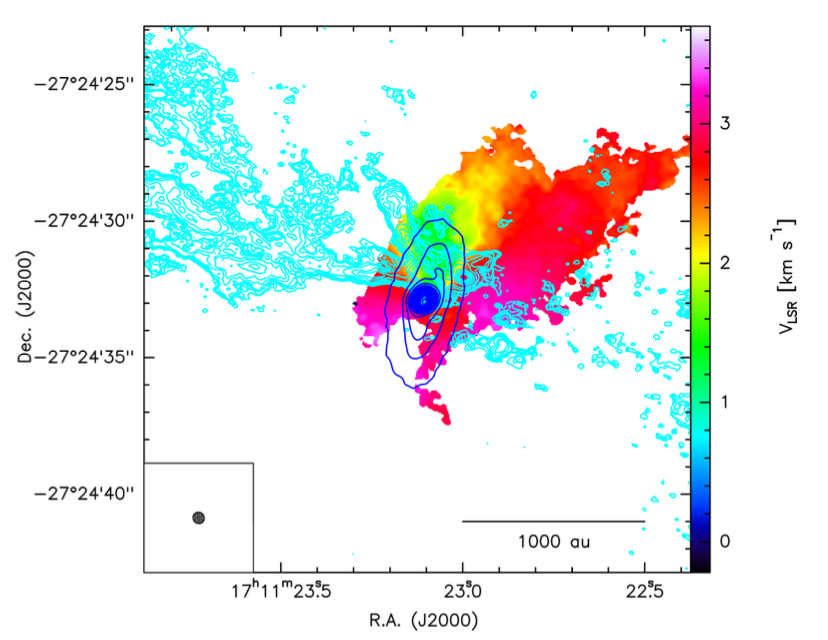
\includegraphics[width=\linewidth, angle=102.3]{observation images/BHB2007 11_b.png}
%         \label{fig: BHB2007 11-1}
%     \end{subfigure}
%     \begin{subfigure}[b]{0.40\linewidth}        %% or \columnwidth
%         \centering
%         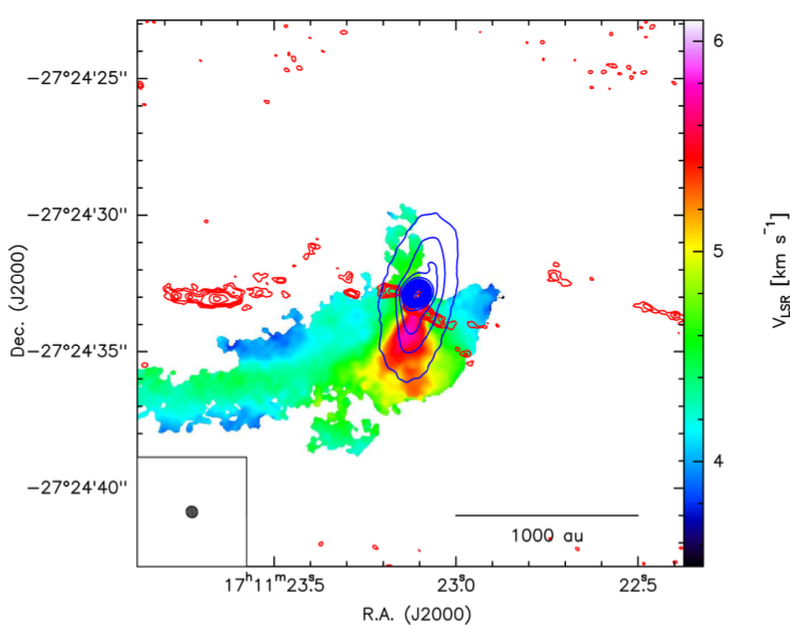
\includegraphics[width=\linewidth, angle=102.3]{observation images/BHB2007 11_r.png}
%         \label{fig: BHB2007 11-2}
%     \end{subfigure}
%     \begin{subfigure}[b]{0.45\linewidth}        %% or \columnwidth
%         \centering
%         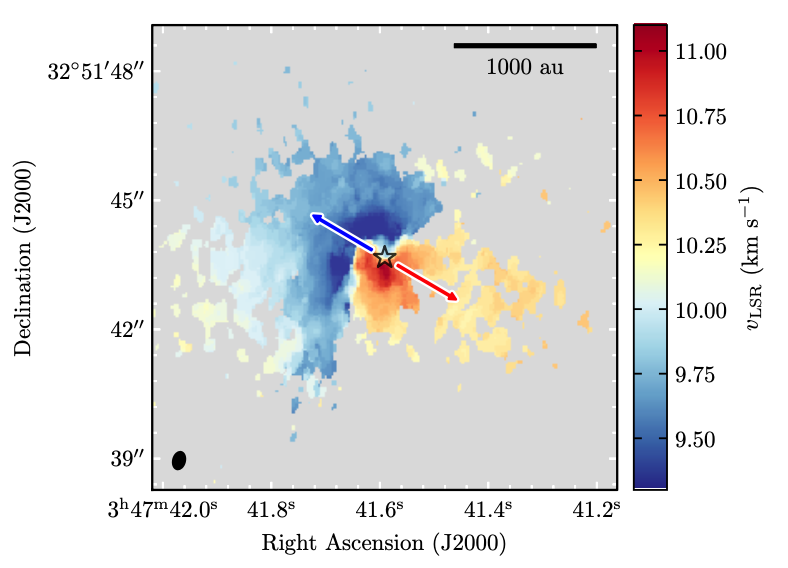
\includegraphics[width=\linewidth, angle=100]{observation images/B5-IRS1.png}
%         \label{fig: B5-IRS1}
%     \end{subfigure}
%     \begin{subfigure}[b]{0.30\linewidth}        %% or \columnwidth
%         \centering
%         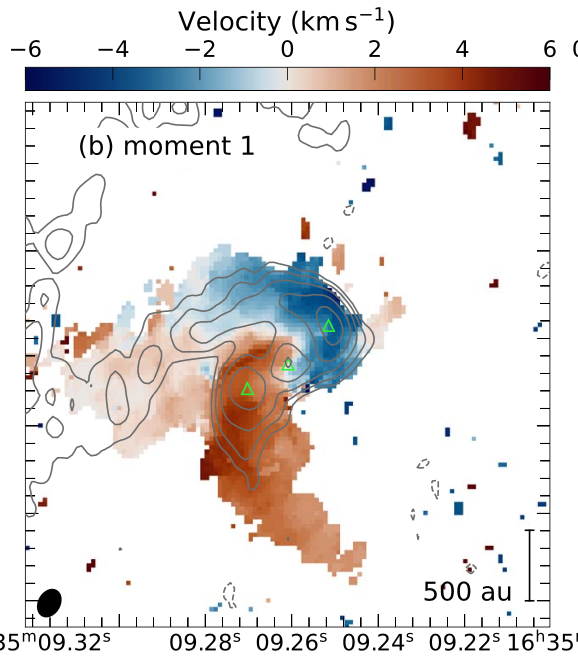
\includegraphics[width=\linewidth, angle=143.5]{observation images/G336.01-0.82.png}
%         \label{fig: G336.01-0.82}
%     \end{subfigure}
%     \begin{subfigure}[b]{0.35\linewidth}        %% or \columnwidth
%         \centering
%         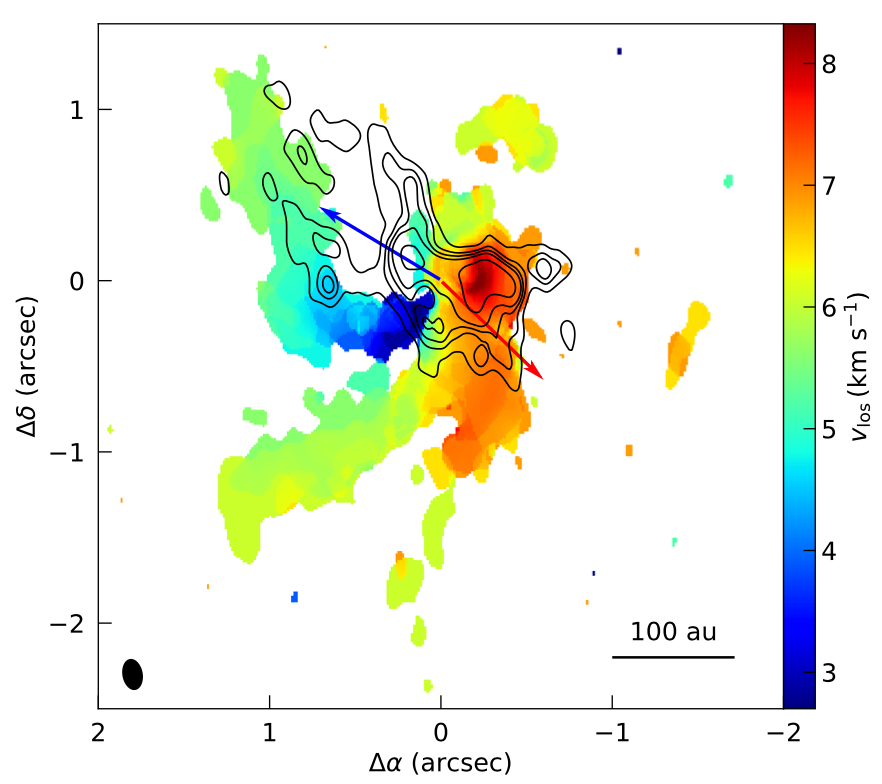
\includegraphics[width=\linewidth, angle=40.2]{observation images/IRAS 04239+2436.png}
%         \label{fig: IRAS 04239+2436}
%     \end{subfigure}
%     \begin{subfigure}[b]{0.40\linewidth}        %% or \columnwidth
%         \centering
%         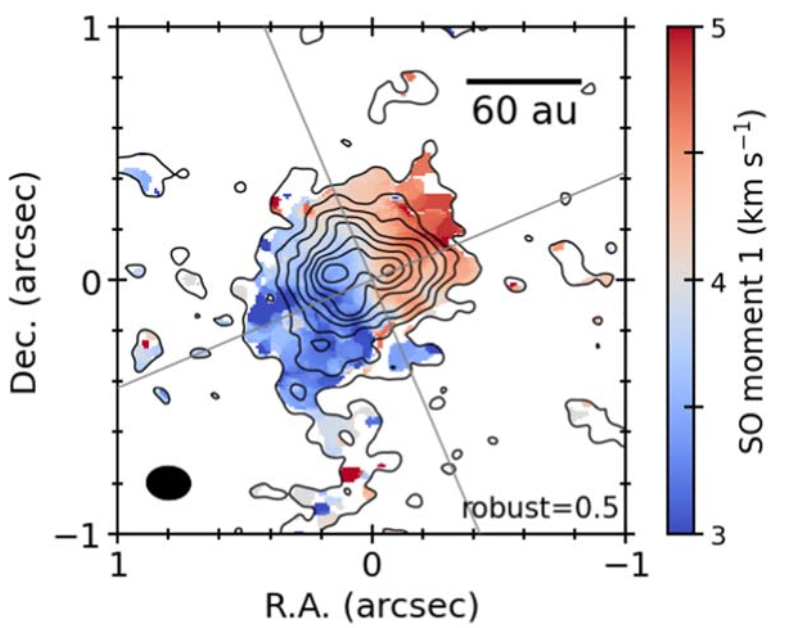
\includegraphics[width=\linewidth, angle=334.7]{observation images/IRAS 16253-2429.png}
%         \label{fig: IRAS 16253-2429}
%     \end{subfigure}
%     \caption{Previous observations
%     \label{fig: Previous observations 1-1}}
% \end{figure*}
% \begin{figure*}
%     \begin{subfigure}[b]{0.40\linewidth}        %% or \columnwidth
%         \centering
%         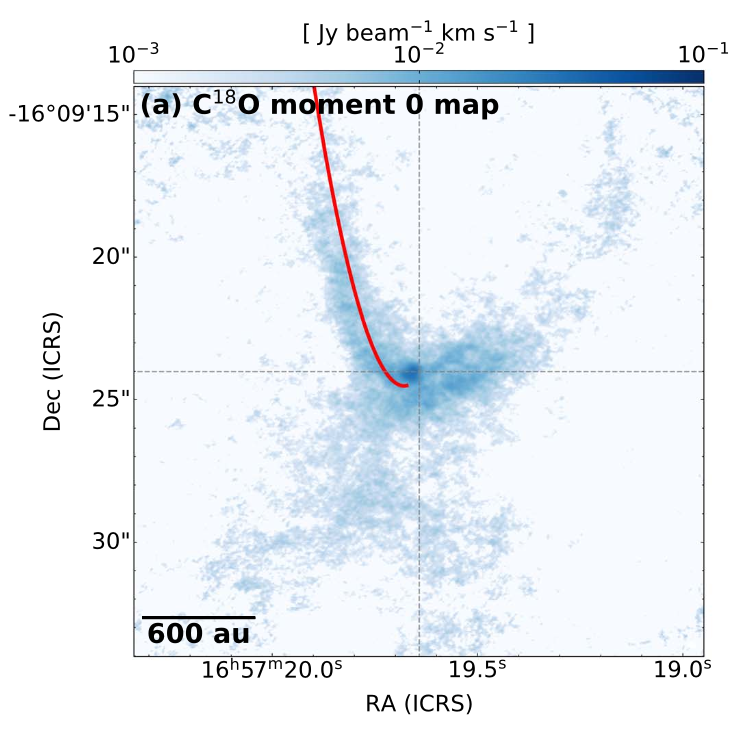
\includegraphics[width=\linewidth]{observation images/IRAS 16544–1604.png}
%         \label{fig: IRAS 16544–1604}
%     \end{subfigure}
%     \begin{subfigure}[b]{0.40\linewidth}        %% or \columnwidth
%         \centering
%         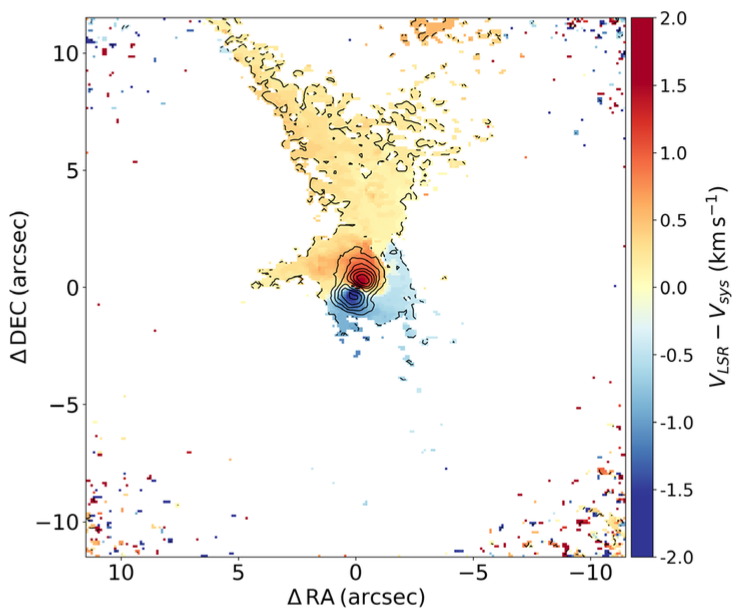
\includegraphics[width=\linewidth, angle=298]{observation images/Oph IRS 63.png}
%         \label{fig: Oph IRS 63}
%     \end{subfigure}
%     \begin{subfigure}[b]{0.40\linewidth}        %% or \columnwidth
%         \centering
%         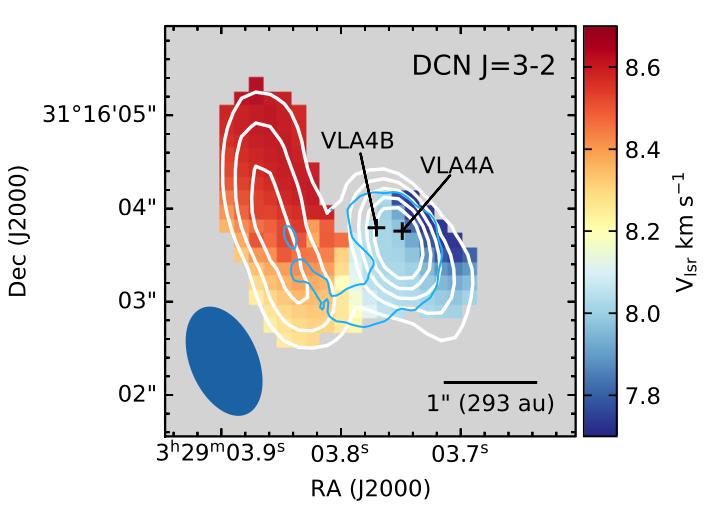
\includegraphics[width=\linewidth, angle=164.4]{observation images/SVS13A.png}
%         \label{fig: SVS13A}
%     \end{subfigure}
%     \begin{subfigure}[b]{0.40\linewidth}        %% or \columnwidth
%         \centering
%         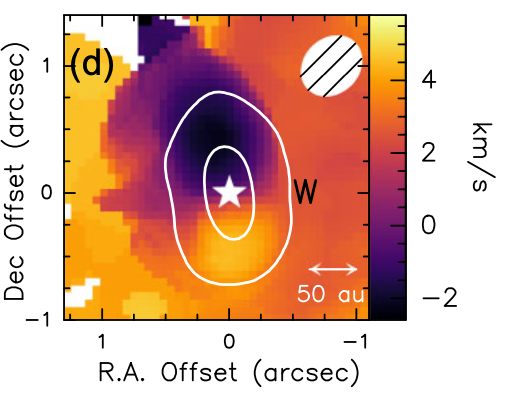
\includegraphics[width=\linewidth, angle=80.2]{observation images/VLA 1623-2417W.png}
%         \label{fig: VLA 1623-2417W}
%     \end{subfigure}
%     \begin{subfigure}[b]{0.40\linewidth}        %% or \columnwidth
%         \centering
%         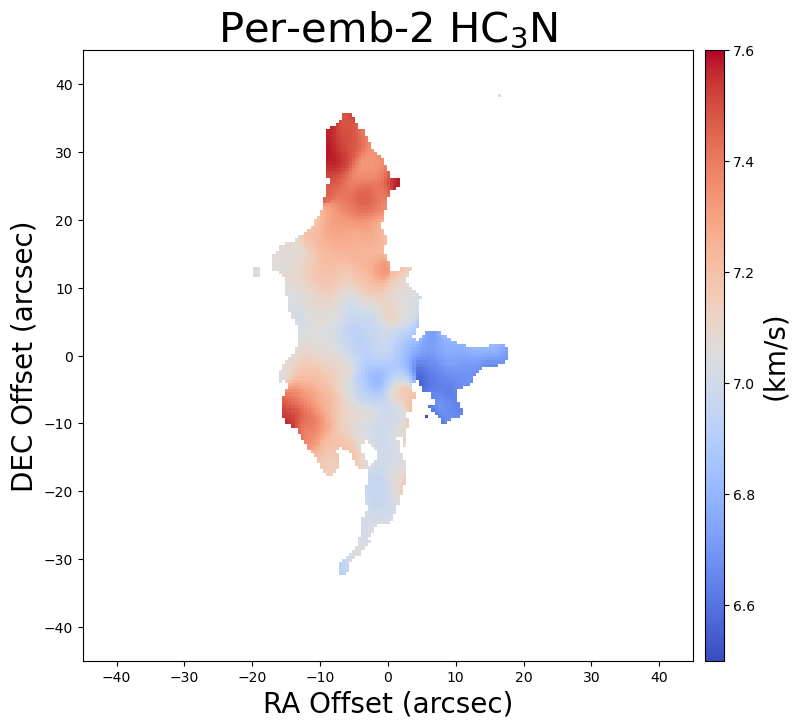
\includegraphics[width=\linewidth, angle=223.6]{observation images/Per_emb_2.png}
%         \label{fig: Per_emb_2}
%     \end{subfigure}
%     \caption{Previous observations
%     \label{fig: Previous observations 1-2}}
% \end{figure*}

